%!TEX root = ../template.tex
%%%%%%%%%%%%%%%%%%%%%%%%%%%%%%%%%%%%%%%%%%%%%%%%%%%%%%%%%%%%%%%%%%%%
%% chapter2.tex
%% NOVA thesis document file
%%
%% Chapter with the template manual
%%%%%%%%%%%%%%%%%%%%%%%%%%%%%%%%%%%%%%%%%%%%%%%%%%%%%%%%%%%%%%%%%%%%

\typeout{NT FILE chapter2.tex}%


\chapter{Background}
\label{cha:Background}

In this chapter we present the necessary background for the formal verification field and the elected tools.

\section{Hoare logic}
\label{sec:Hoare_logic}

Hoare Logic is a formal system for reasoning about the correctness of computer programs. However, 
computer arithmetic often differs from the standard arithmetic familiar to mathematicians due to issues like finite 
precision, overflows, and machine-specific behaviors. To account for these differences, C.A.R. Hoare introduced a new logic
based on assertions and inference rules for reasoning about the partial correctness of programs. Drawing inspiration 
from mathematical axioms and formal proof techniques, he proposed a framework where program behavior could be specified 
and verified using logical formulas. This laid the foundation for systematic program verification and emphasized the need 
to model computational constraints, such as those arising from the limitations of machine arithmetic, within a formal system.

"The purpose of this study is to provide a logical basis for proofs of the properties of a program"~\cite{Hoare69}.

\subsection{Hoare Triples}

The main construction of Hoare logic is the \textit{Hoare triple}, where $P$ is a pre-condition, $C$ is a program (fragment) 
and $Q$ is a post-condition:

\[ 
  \{P\}C\{Q\}
\]

A Hoare triple expresses a partial correctness guarantee: if the precondition $P$ holds before executing a program fragment 
$C$, and if $C$ terminates, then the postcondition $Q$ will hold afterward. This is a partial correctness result since the 
termination of $C$ is not assured by the triple. Total correctness is achieved when termination is also guaranteed.

\subsection{Assignment Axiom}

\[ 
  \inferrule
  { \ }
  {\{P_0\} \ \textit{x} := \textit{f} \ \{P\}}
  \quad (assign)
\]

where $x$ is a variable identifier; $f$ is an expression; $P_0$ is obtained from $P$ by substituting $f$ for all occurrences 
of $x$.

The axiom expresses that to prove a postcondition $P$ holds after assigning the expression $f$ to the variable $x$,
it suffices to prove the precondition $P_0$ before the assignment, where $P_0$ is obtained by substituting every occurrence of
$x$ in $P$ with the expression $f$.

\subsection{Rule of Composition}

The inference rule for composition states that if the postcondition of the first program segment matches the precondition 
of the second, then the entire program will produce the intended result—assuming the initial precondition of the first 
segment holds.

\[ 
  \inferrule
  {P \{ Q_1 \} R_1 \quad \quad  R_1 \{ Q_2 \} R}
  {P \{ (Q_1 ; Q_2) \} R} 
  \quad (composition)
\]

Hoare Logic was significantly strengthened by Cook's seminal work on the soundness and completeness of an axiom system 
for program verification. In his paper, Cook presented a Hoare-style axiom system tailored to a simple programming language 
and rigorously established both its soundness and adequacy. He concluded that, under reasonable assumptions, Hoare Logic is 
not only intuitively effective but also formally complete as a system for reasoning about program correctness~\cite{0207005}.

After setting an elegant axiomatic framework for reasoning about program correctness through the use of Hoare triples 
$\{P\}C\{Q\}$, its practical application in large-scale or automated verification tasks presents significant challenges. 
Chief among these is the burden of manually identifying appropriate preconditions and invariants. To address this, 
Edsger W. Dijkstra introduced the weakest precondition calculus, which reformulates program correctness into a computational 
problem: given a command $C$ and a desired postcondition $Q$, the function $wp(C,Q)$ computes the weakest precondition $P$ 
such that $\{P\}C\{Q\}$ holds~\cite{Dijkstra76}.

This transformation from proof obligations to a calculable precondition function represents a critical step toward automating 
program verification. Unlike Hoare's original formulation, which requires deductive reasoning to derive correctness properties, 
weakest precondition semantics allow for algorithmic generation of verification conditions, thereby enabling integration 
with automated theorem provers and SMT solvers.

The influence of weakest preconditions is particularly evident in modern deductive verification tools such as \whythree
~\cite{boogie11why3}, and \textsf{Dafny}~\cite{Leino10}.

\section{OCaml}
\label{sec:OCaml}

OCaml is a statically typed functional programming language rooted in the ML family, originally developed 
to serve as the implementation language for theorem provers such as LCF. It inherits the foundational principles 
of typed $\lambda$-calculus, formal logic, and abstract interpretation, and extends them through practical language design 
aimed at enabling both expressiveness and efficiency~\cite{FilliatrePereiraSousa2018}.

First released in the mid-1990s, OCaml is the principal evolution of the Caml dialect of the ML family. The name OCaml, 
originally short for Objective Caml, reflects the addition of object-oriented features to the Caml language. While Caml 
stood for Categorical Abstract Machine Language, OCaml moved away from its dependence on the original abstract machine 
model~\cite{leroy:inria-00070049}. The language is primarily developed and maintained by INRIA, which continues to guide 
its implementation and evolution.

OCaml distinguishes itself from many academically inspired languages through its strong emphasis on performance. Its static 
type system eliminates the need for runtime type checking by ensuring type correctness at compile time, thereby avoiding the 
performance overhead commonly associated with dynamically typed languages. This design enables OCaml to maintain high 
execution efficiency while preserving strong safety guarantees at runtime. Exceptions to this safety model arise only in 
specific low-level scenarios, such as when array bounds checking is explicitly disabled or when employing type-unsafe features 
like runtime serialization~\cite{FilliatrePereiraSousa2018}.

For the standard compiler toolchain features, \ocaml has both a high-performance native-code compiler (\textsf{ocamlopt}) and a 
bytecode compiler (\textsf{ocamlc}). The native-code compiler produces efficient machine code via a sophisticated optimizing 
backend~\cite{abs-1011-1783}, while the bytecode compiler offers portability and rapid development. Both compilers are integrated 
with a runtime system that supports automatic memory management via a garbage collector and provides facilities for exception handling, 
concurrency, and system interaction.

\subsection{Immutability by default}

Immutability is promotted as a default design principle in this language. Rather than modifying existing values, new ones 
are created through expression evaluation. This absence of mutable shared state simplifies reasoning about program behavior 
and eliminates many common sources of verification complexity, such as aliasing and unintended side effects.

\begin{ocamlenv}
  let x = 5
  let y = x + 1 (* x is not modified, just referenced *)
\end{ocamlenv}

Since values are not modified in place, program semantics are preserved under substitution, facilitating referential transparency, 
making symbolic execution and logical reasoning over programs more straightforward in deductive verification.

\subsection{ADTs (Algebraic Data Types)}

In \ocaml, data types fall into three broad categories: atomic predefined types (e.g., \texttt{int}, \texttt{bool}), type 
constructors provided by the language (e.g., \texttt{list}, \texttt{array}, \texttt{option}), and user-defined types, which 
are declared through the general mechanism of algebraic data types, for instance:

\begin{ocamlenv}
  type 'a tree =
    | Leaf
    | Node of 'a tree * 'a * 'a tree
\end{ocamlenv}

ADTs support exhaustive pattern matching, which is particularly useful for enabling structural recursion and inductive reasoning.
From a verification perspective, this ensures all possible cases are covered, making formal reasoning both precise and complete. 
Such properties are essential for theorem proving and are readily leveraged by formal tools like \gospel, Coq, and \whythree.

\subsection{First-Class and Higher-Order Functions}

\ocaml treats functions as first-class values: they can be passed as arguments, returned from other functions, 
and stored in data structures. Combined with lexical scoping and immutable data, this makes \ocaml particularly 
well-suited for working with higher-order abstractions, a feature that aligns naturally with formal systems based on 
higher-order logic.

\begin{ocamlenv}
  let apply_twice f x = f (f x)

  let square x = x * x

  let result = apply_twice square 2  (* returns 16 *)
\end{ocamlenv}

In the context of deductive verification, such functional abstractions support elegant formulations of parametric specifications 
and reasoning principles.

\subsection{Modules, Functors and Signatures}

The module system enables parametric modularity through modules and functors, supporting abstraction, separation of concerns, and 
scalable design. At the heart of this system are signatures, which serve as formal interfaces specifying the types and values a 
module must provide while hiding the implementation details. These signatures play a key role in formal verification by allowing 
reasoning about components based solely on their interfaces, without depending on how they are implemented.

\begin{ocamlenv}
  module type StackSig = sig
    type 'a t
    val empty : 'a t
    val push : 'a -> 'a t -> 'a t
    val pop : 'a t -> 'a t
  end

  module Stack : StackSig = struct
    type 'a t = 'a list
    let empty = []
    let push x s = x :: s
    let pop = function [] -> [] | _ :: tl -> tl
  end

  module type ElemSig = sig type t end

  module MakeStack (_ : ElemSig) : StackSig = Stack
\end{ocamlenv}

This modular structure is especially useful in verification contexts because it clearly separates the interface from the 
implementation. This separation makes it easier to reason about and verify each component independently, improving 
maintainability and correctness.

\subsection{Type Abstraction and Encapsulation}

One of \ocaml's strengths lies in its support for abstract types via module signatures. This allows developers to hide 
implementation details and expose only essential operations, enabling verification at the level of observable behavior rather 
than internal representation.

\begin{ocamlenv}
  module Counter : sig
    type t
    val create : unit -> t
    val incr : t -> t
    val get : t -> int
  end = struct
    type t = int
    let create () = 0
    let incr x = x + 1
    let get x = x
  end
\end{ocamlenv}

By hiding the concrete type \texttt{int}, this interface prevents misuse and allows formal specification to focus solely on 
observable behavior. In verification tools, this maps cleanly to abstract state machines and promotes reasoning over 
behavior instead of implementation details.

%%modulos assinaturas functors

%%https://arxiv.org/pdf/1011.1783 (native compiler JIT)
%%https://inria.hal.science/inria-00070049v1/document
%%https://usr.lmf.cnrs.fr/lpo/lpo.pdf
%%https://hal.science/hal-01783851v1/file/main.pdf

\section{Standard ML}
\label{sec:Standard_ML}

Standard ML is a functional programming language that fully embraces the expressiveness of mathematical functions. 
However, it was also shaped by practical programming needs, leading to the inclusion of imperative constructs and a 
robust exception handling system. The language supports modularity through an advanced system of parametric modules, 
designed to facilitate the structured development of large-scale software systems. Moreover, Standard ML is strongly 
and statically typed, and it was the first programming language to introduce a form of polymorphic type inference that 
combines strong type safety with considerable flexibility in programming style ~\cite{milner1997definition}.

One of the most distinguishing features of Standard ML is its formal definition, which precisely specifies the language's 
static and dynamic semantics using structural operational semantics (SOS). This operational style makes the semantics 
especially suitable for mechanization in proof assistants like HOL, bridging the gap between theoretical definitions 
and executable verification. This made it one of the first programming languages to be fully defined in a mathematical 
sense, laying a strong foundation for formal verification frameworks and verified compilers such as 
CakeML~\cite{milner1997definition, SewellMTKMAO23}. 

Even though the foundational formal definition of Standard ML had already been established, the ability to embed and 
reason about its semantics within a proof assistant like HOL marked a significant advance. This transformation from a 
descriptive, paper based semantics to one that is executable and machine-verifiable played a key role in laying the 
groundwork for end-to-end verified compilers~\cite{Syme93}.

\section{Why3}
\label{sec:Why3}

\whythree is the successor to the Why verification platform, offering a rich first-order language and a highly configurable 
toolchain for generating proof obligations in multiple formats. Its development is driven by the need to model both purely 
functional and imperative program behaviors and to formally verify their properties. Since verifying non-trivial programs 
typically requires abstracting them into pure logical models, \whythree is designed to bridge the gap between practical programming 
constructs and formal reasoning frameworks.

\whythree introduces \whyml, a specification and programming language that serves both as an expressive front-end and as 
an intermediate language for verifying programs written in other languages such as C, Java, and Ada.~\cite{FilliatreP13} 
It supports rich language features including pattern matching, recursive definitions, algebraic data types, and inductive or 
coinductive predicates. Moreover, it comes with a standard library of logical theories covering arithmetic, sets, maps, 
and more.

\whythree sets itself apart from other approaches that also provide rich specification languages like \textsf{Coq} and 
\textsf{Isabelle} by aiming to maximize automation. Rather than functioning as a standalone theorem prover, it serves 
as a front-end that generates proof obligations to be discharged by external automated provers such as Z3, Alt-Ergo, 
Vampire, and CVC4, as well as interactive systems like Coq and PVS.

In the context of automated program verification, \whythree simplifies the process by automatically generating verification 
conditions from annotated source code and delegating their resolution to a variety of powerful external theorem provers. 
When certain features (e.g., polymorphic types or pattern matching) are not supported by a backend prover, \whythree automatically 
applies transformations to encode them into a compatible form. This architecture allows developers to focus on writing 
correct specifications while benefiting from automation in proving correctness properties.~\cite{boogie11why3}

\section{GOSPEL and Cameleer}
\label{sec:Cameleer}

The evolution of deductive verification and proof automation has progressed significantly over the years. Recently, a 
combination of tools has been developed to apply these technologies to \ocaml, a language that has not been widely explored in 
this context~\cite{PereiraR20}. The need for a verification framework was addressed with the introduction of \cameleer, a tool 
for the deductive verification of programs written in \ocaml, whose main objective is the automatic proof of functional code. 
However, \cameleer alone, using only standard \ocaml, cannot perform these proofs. To enable verification, \gospel specifications 
must be added to the \ocaml code.

\gospel terms are defined using the semantics of Separation Logic and are applied to \ocaml interfaces. The acronym \gospel stands 
for “Generic OCaml Specification Language,” indicating that the specification logic is not limited to a single tool but is intended 
for a variety of uses, such as verification, testing, and informal documentation~\cite{ChargueraudFLP19}. Unlike other behavioural 
specification languages such as \textsf{SPARK} and \textsf{JML}, \gospel supports Separation Logic, a significant extension of Hoare 
Logic and a powerful framework for reasoning about real-world programs~\cite{Reynolds02, OHearnRY01}. While \gospel is not the first 
tool to use Separation Logic, it uniquely introduces implicit permission association in data types, a feature not found in tools 
like \textsf{VeriFast} or \textsf{Viper}~\cite{ChargueraudFLP19}.

\cameleer takes as input an \ocaml program annotated with \gospel specifications and translates it into \whyml, the intermediate 
language used by the \whythree platform. Once translated, the code can be processed by \whythree, which leverages a range of automated 
theorem provers, such as Alt-Ergo, Z3, and CVC5, to discharge verification conditions. This seamless integration between \cameleer, 
\gospel, and \whythree significantly enhances the level of proof automation, allowing developers to verify functional correctness 
properties of \ocaml programs with minimal manual intervention. This behaviour is captured by the following pipeline:

\begin{figure}[H]
    \centering
    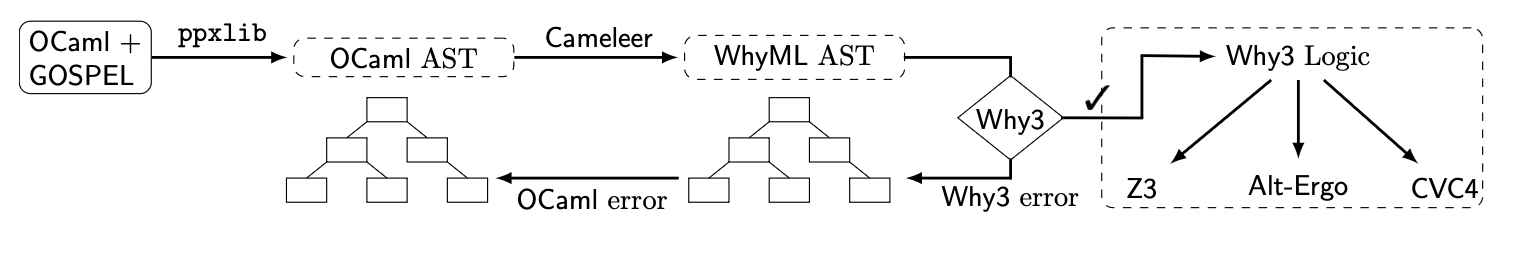
\includegraphics[width=\linewidth]{images/Cameleer_From_Paper.png}
    \caption{The Original Cameleer Pipeline~\cite{PereiraR20}}
    \label{fig:CameleerPipeline}
\end{figure}

In figure \ref{fig:CameleerPipeline} demonstrates how the translation mechanism integrates with surrounding frameworks to produce 
deductively verified \ocaml code annotated with \gospel specifications. If an error is detected in the original \ocaml code during 
translation, the process reverts to the source, requiring corrections to ensure that the generated \whyml code is syntactically and 
semantically valid. Within the \whythree tool, if the generated verification goals cannot be discharged by the automated provers, it indicates 
that the specifications may be imprecise or incomplete and require refinement. These issues are highlighted by the tool, guiding the 
user to improve the annotations. Once all verification conditions are successfully proven, the resulting program is guaranteed to 
be free from compiler-introduced bugs or errors, ensuring a high level of formal correctness~\cite{Filliatre11}.

Lets take this simple example for an iterative factorial in \ocaml + \gospel after applying the \cameleer tool:

\begin{gospell}
(*@ 
  function rec factorial (n:int) :int = 
    if n=0 then 1 else n * factorial (n-1)
*)
(*@ 
  requires n >= 0
  variant n
*)
let fact n = 
  let r = ref 1 in 
    for i=1 to n do 
      (*@invariant !r = factorial (i-1)*)
      r := !r*i 
    done; 
    !r
(*@ 
  r = fact n
  requires n >= 0 
  ensures r = factorial n
*)
\end{gospell}

The translated code to \whyml creates 2 goals, one for the function \inlinecode{fact} and another for the logical function
\inlinecode{factorial}. After splitting the goals we get for \inlinecode{fact} the variant and pre-condition, and for
\inlinecode{factorial} the invariant initialization, the invariant preservation, the post-condition and the VC:

\begin{figure}[H]
    \centering
    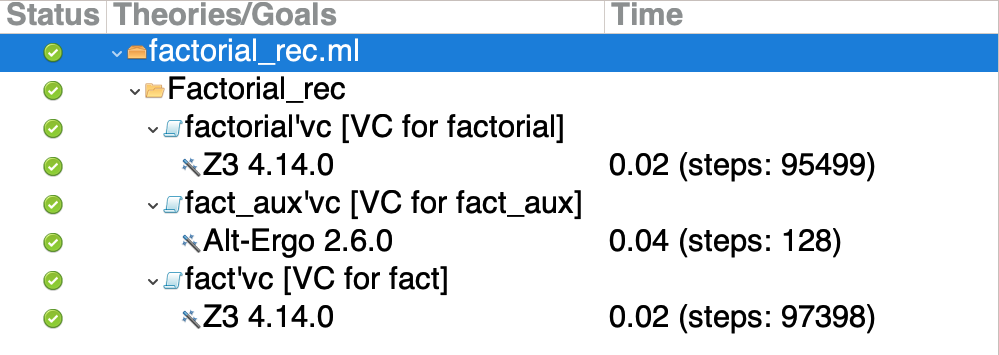
\includegraphics[width=0.6\linewidth]{images/Why3Goals.png}
    \caption{The Goals Proved in \whythree}
    \label{fig:Why3Goals}
\end{figure}

All verification goals were successfully discharged in figure \ref{fig:Why3Goals} through the automated provers, resulting in the 
original \ocaml code, annotated 
with \gospel specifications, being fully verified. This outcome demonstrates the effectiveness of the verification pipeline, 
where the combination of \cameleer and \whythree enables high levels of automation in proving the functional correctness of 
\ocaml programs.